\chapter{Probas}
\label{chap:probas}

As probas realizáronse co obxectivo de comprobar o funcionamento da \gls{api} e da aplicación móbil, tanto de maneira illada como na súa integración. Para iso combináronse probas unitarias, de integración e de interface con comprobacións manuais en dispositivos Android, avaliando a lóxica de procesamento e validación dos datos, a persistencia, os servizos, os principais fluxos da aplicación e o tratamento de erros e casos límite.

A Táboa~\ref{tab:matriz-probas} resume os distintos tipos de probas realizadas, as ferramentas empregadas e os principais aspectos comprobados. O detalle das probas e as evidencias da súa execución recóllense no Apéndice~\ref{app:probas-complementarias}.

\begin{table}[htbp]
    \centering
    \small
    \caption{Relación entre os tipos de proba e os aspectos comprobados}
    \label{tab:matriz-probas}

    \setlength{\tabcolsep}{5pt}
    \renewcommand{\arraystretch}{1.15}

    \begin{tabularx}{\textwidth}{
        >{\raggedright\arraybackslash}p{0.20\textwidth}
        >{\raggedright\arraybackslash}p{0.26\textwidth}
        >{\raggedright\arraybackslash}X
    }
        \hline
        \textbf{Tipo} &
        \textbf{Ferramentas} &
        \textbf{Aspectos comprobados} \\
        \hline

        Unitarias da API &
        unittest &
        Procesamento de datas e doses, cálculo da confianza, validación do INR e funcións auxiliares. \\

        Integración da API &
        TestClient, MagicMock &
        Endpoints, respostas HTTP, extracción, preprocesamento, notificacións e dependencias externas. \\

        Unitarias do cliente &
        flutter\_test &
        Modelos, modelos de vista, métricas de cumprimento e planificación de recordatorios. \\

        Servizos do cliente &
        MockClient, AES-GCM &
        Comunicación HTTP, tratamento de erros, cifrado e integridade das mensaxes. \\

        Persistencia &
        SQLite &
        Gardado e recuperación de pautas, estados das tomas, reimportación e información das persoas supervisadas. \\

        Interface &
        testWidgets &
        Navegación, formularios, estados de carga, calendario, progreso e mensaxes de erro. \\

        Manuais &
        Dispositivos Android &
        Cámara, galería, PDF, permisos, QR, notificacións e sincronización entre dispositivos. \\
        \hline
    \end{tabularx}
\end{table}

\section{Probas unitarias}
As probas unitarias permiten verificar compoñentes concretos de maneira illada, empregando entradas coñecidas e comprobando que a saída obtida sexa a esperada.

Na \gls{api} utilizouse o módulo \textit{unittest} de Python. Probáronse as funcións de limpeza e normalización de datas, a interpretación das doses, o cálculo da confianza media e as regras de validación de valores como o \gls{inr}.

No cliente empregouse \textit{flutter\_test} para comprobar os modelos de datos, a conversión do \gls{json} devolto pola \gls{api}, a edición e validación das pautas e o cálculo das métricas de cumprimento. Tamén se probaron os modelos de vista e a lóxica encargada de determinar cando unha dose debe xerar un recordatorio. Para estas probas empregáronse datas e horas fixas, evitando que os resultados dependan do momento de execución.

Por último, o servizo de cifrado probouse mediante operacións reais con \gls{aesgcm}, verificando o descifrado coa clave correcta e o rexeitamento de mensaxes alteradas ou cifradas cunha clave diferente.

\section{Probas de integración}

As probas de integración permitiron comprobar o funcionamento conxunto dos diferentes compoñentes do sistema.

Na \gls{api} empregouse TestClient para realizar peticións aos distintos endpoints. As chamadas a servizos externos, como Azure Document Intelligence, Firebase e Key Vault, simuláronse para poder probar diferentes respostas e situacións de erro de maneira controlada. Comprobáronse os endpoints de extracción, preprocesamento, centros sanitarios, notificacións e saúde, verificando tanto os casos correctos como as distintas respostas de erro.

No cliente comprobouse a comunicación coa \gls{api} e a persistencia dos datos en SQLite. Probouse, entre outros casos, que unha folla de tratamento pode gardarse e recuperarse correctamente, que ao importar de novo a mesma folla se conservan as tomas xa confirmadas e que unha nova folla actualiza correctamente a pauta. Tamén se verificaron fluxos que combinan a captura e gardado dun informe, a planificación dos recordatorios e a sincronización coa persoa supervisora.

\section{Probas de interface e usabilidade}

As probas de interface permitiron comprobar o comportamento das principais pantallas da aplicación e a resposta ante as accións da persoa usuaria. Verificáronse aspectos como a navegación, os formularios, os estados de carga, as mensaxes de erro e pantallas como a revisión da pauta, o calendario, o progreso e a configuración. Para iso simuláronse interaccións como pulsacións ou introdución de datos e comprobouse que a interface mostrase o resultado esperado.

Estas probas automatizadas complementáronse con probas manuais en dispositivos Android. Comprobáronse os principais fluxos da aplicación, como a incorporación dunha folla desde a cámara, a galería ou un documento \gls{pdf}, a revisión e corrección dos datos extraídos, a vinculación mediante código \gls{qr}, a recepción de notificacións e a sincronización entre dous teléfonos. Tamén se probaron situacións de erro para comprobar que as mensaxes mostradas pola aplicación fosen claras e comprensibles.

Estas comprobacións permitiron avaliar a usabilidade básica da aplicación, aínda que non se realizou un estudo formal con participantes externos.

\section{Resultados e cobertura}

A \gls{api} obtivo unha cobertura global do 96,1 \%. Como pdodemos ver na Figura~\ref{fig:cobertura-componentes} todos os seus módulos alcanzaron o 100 \%, agás o de preprocesamento, cun 93,6 \%. Neste módulo quedaron sen executar algunhas ramas correspondentes a casos específicos e situacións de erro pouco habituais.

No cliente obtívose unha cobertura global do 72,8 \%. Os modelos acadaron o 100 \%, os modelos de vista o 81,6 \% e os widgets incluídos nas probas o 78,9 \%. Os servizos \gls{http}, a persistencia en SQLite e o servizo de cifrado superaron o 99 \% de cobertura.

A menor cobertura global do cliente débese principalmente a funcionalidades que dependen directamente de servizos e características propias do dispositivo, especialmente a sincronización mediante Firebase e a xestión das notificacións locais. Estas partes non poden comprobarse completamente mediante o contorno habitual de probas de Flutter, polo que o seu funcionamento verificouse tamén mediante as probas manuais realizadas nos dispositivos Android. Ademais, determinados fluxos de interface relacionados coa cámara e coa vinculación requiren interaccións co dispositivo, o que tamén reduce a cobertura obtida mediante as probas automatizadas.

\begin{figure}[htbp]
    \centering
    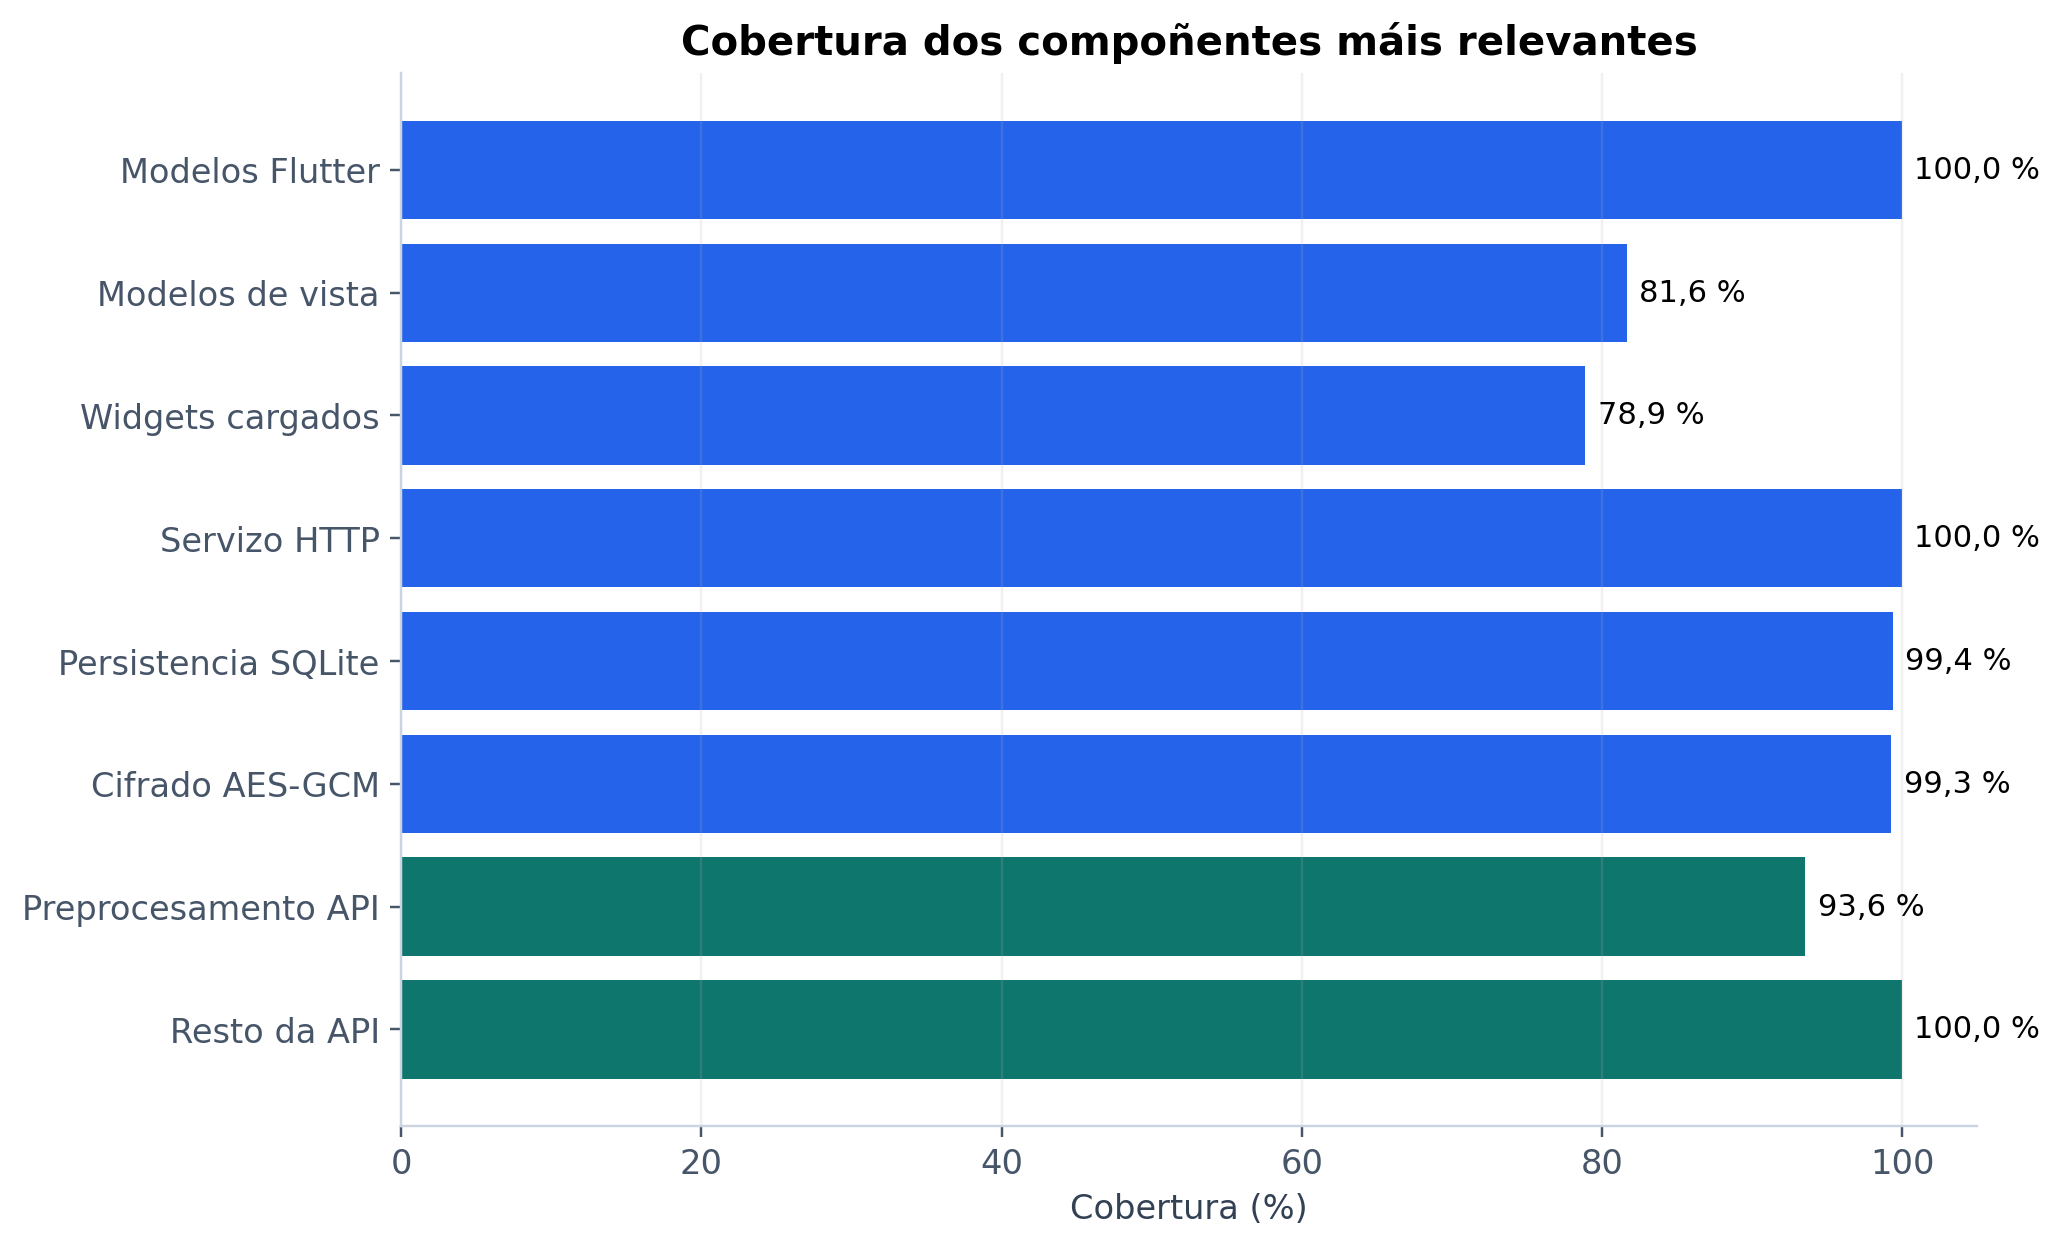
\includegraphics[
        width=\textwidth
    ]{imaxes/09-Probas/cobertura-componentes.png}
    \caption{Cobertura dos principais compoñentes da solución}
    \label{fig:cobertura-componentes}
\end{figure}

